\documentclass[10pt,twocolumn]{article}

\usepackage[letterpaper,margin=0.72in]{geometry}
\usepackage[T1]{fontenc}
\usepackage[utf8]{inputenc}
\usepackage{times}
\usepackage{microtype}
\usepackage{graphicx}
\usepackage{booktabs}
\usepackage{amsmath}
\usepackage{amssymb}
\usepackage{caption}
\usepackage[numbers,sort&compress]{natbib}
\usepackage[colorlinks=true,citecolor=blue,linkcolor=blue,urlcolor=blue]{hyperref}
\usepackage{balance}
\usepackage{stfloats}
\usepackage{xcolor}

\graphicspath{{figures/}}
\newcommand{\AccGemma}{67\%}
\newcommand{\AccLlama}{63\%}
\newcommand{\AccLlamaSmall}{48\%}
\newcommand{\AccQwen}{58\%}
\newcommand{\AnatInGivenGemma}{56\%}
\newcommand{\AnatInGivenLlama}{45\%}
\newcommand{\AnatInGivenLlamaSmall}{57\%}
\newcommand{\AnatInGivenQwen}{58\%}
\newcommand{\AnatInGoldGemma}{20\%}
\newcommand{\AnatInGoldLlama}{28\%}
\newcommand{\AnatInGoldLlamaSmall}{19\%}
\newcommand{\AnatInGoldQwen}{20\%}
\newcommand{\AnatWrongNGemma}{364}
\newcommand{\AnatWrongNLlama}{343}
\newcommand{\AnatWrongNLlamaSmall}{512}
\newcommand{\AnatWrongNQwen}{472}
\newcommand{\AucBothGemma}{0.72}
\newcommand{\AucBothLlama}{0.77}
\newcommand{\AucBothLlamaSmall}{0.84}
\newcommand{\AucBothQwen}{0.74}
\newcommand{\AucConfGemma}{0.50}
\newcommand{\AucConfLlama}{0.69}
\newcommand{\AucConfLlamaSmall}{0.61}
\newcommand{\AucConfQwen}{0.60}
\newcommand{\AucGainHiGemma}{0.29}
\newcommand{\AucGainHiLlama}{0.13}
\newcommand{\AucGainHiLlamaSmall}{0.32}
\newcommand{\AucGainHiQwen}{0.19}
\newcommand{\AucGainLoGemma}{0.15}
\newcommand{\AucGainLoLlama}{0.04}
\newcommand{\AucGainLoLlamaSmall}{0.16}
\newcommand{\AucGainLoQwen}{0.08}
\newcommand{\AucGeoGemma}{0.73}
\newcommand{\AucGeoLlama}{0.75}
\newcommand{\AucGeoLlamaSmall}{0.83}
\newcommand{\AucGeoQwen}{0.74}
\newcommand{\CrossModelMax}{88\%}
\newcommand{\CrossModelMin}{66\%}
\newcommand{\CrossModelPairs}{12}
\newcommand{\ErrNGemma}{364}
\newcommand{\ErrNLlama}{339}
\newcommand{\ErrNLlamaSmall}{488}
\newcommand{\ErrNQwen}{463}
\newcommand{\HintEndGemma}{43\%}
\newcommand{\HintEndLlama}{54\%}
\newcommand{\HintEndLlamaSmall}{10\%}
\newcommand{\HintEndQwen}{29\%}
\newcommand{\HintMisledNGemma}{53}
\newcommand{\HintMisledNLlama}{57}
\newcommand{\HintMisledNLlamaSmall}{107}
\newcommand{\HintMisledNQwen}{69}
\newcommand{\HintPeakDepthGemma}{0.48}
\newcommand{\HintPeakDepthLlama}{0.47}
\newcommand{\HintPeakDepthLlamaSmall}{0.25}
\newcommand{\HintPeakDepthQwen}{0.46}
\newcommand{\HintPeakGemma}{64\%}
\newcommand{\HintPeakLlama}{84\%}
\newcommand{\HintPeakLlamaSmall}{69\%}
\newcommand{\HintPeakQwen}{70\%}
\newcommand{\HintResistEndGemma}{100\%}
\newcommand{\HintResistEndLlama}{99\%}
\newcommand{\HintResistEndLlamaSmall}{59\%}
\newcommand{\HintResistEndQwen}{96\%}
\newcommand{\LayersGemma}{42}
\newcommand{\LayersLlama}{32}
\newcommand{\LayersLlamaSmall}{16}
\newcommand{\LayersQwen}{28}
\newcommand{\LineMseGemma}{0.290}
\newcommand{\LineMseLlama}{0.137}
\newcommand{\LineMseLlamaSmall}{0.198}
\newcommand{\LineMseQwen}{0.422}
\newcommand{\NFacts}{2,256}
\newcommand{\NFactsBuilt}{2,273}
\newcommand{\NPromptsPerModel}{16,294}
\newcommand{\NRewrites}{4,323}
\newcommand{\NoWordsGemma}{91\%}
\newcommand{\NoWordsLlama}{94\%}
\newcommand{\NoWordsLlamaSmall}{85\%}
\newcommand{\NoWordsQwen}{90\%}
\newcommand{\OnsetGemma}{0.62}
\newcommand{\OnsetLayerGemma}{26}
\newcommand{\OnsetLayerLlama}{15}
\newcommand{\OnsetLayerLlamaSmall}{10}
\newcommand{\OnsetLayerQwen}{20}
\newcommand{\OnsetLlama}{0.47}
\newcommand{\OnsetLlamaSmall}{0.62}
\newcommand{\OnsetQwen}{0.71}
\newcommand{\PeakGemma}{92\%}
\newcommand{\PeakLlama}{94\%}
\newcommand{\PeakLlamaSmall}{86\%}
\newcommand{\PeakQwen}{92\%}
\newcommand{\PushEarlyGemma}{0\%}
\newcommand{\PushEarlyLlama}{0\%}
\newcommand{\PushEarlyLlamaSmall}{1\%}
\newcommand{\PushEarlyQwen}{0\%}
\newcommand{\PushGoldGemma}{97\%}
\newcommand{\PushGoldLlama}{97\%}
\newcommand{\PushGoldLlamaSmall}{83\%}
\newcommand{\PushGoldQwen}{94\%}
\newcommand{\PushLayerGemma}{38}
\newcommand{\PushLayerLlama}{29}
\newcommand{\PushLayerLlamaSmall}{14}
\newcommand{\PushLayerQwen}{25}
\newcommand{\PushMisledGemma}{96\%}
\newcommand{\PushMisledLlama}{93\%}
\newcommand{\PushMisledLlamaSmall}{74\%}
\newcommand{\PushMisledQwen}{86\%}
\newcommand{\PushNGemma}{192}
\newcommand{\PushNLlama}{121}
\newcommand{\PushNLlamaSmall}{224}
\newcommand{\PushNQwen}{233}
\newcommand{\PushOtherGemma}{95\%}
\newcommand{\PushOtherLlama}{85\%}
\newcommand{\PushOtherLlamaSmall}{82\%}
\newcommand{\PushOtherQwen}{83\%}
\newcommand{\PushRandomGemma}{4\%}
\newcommand{\PushRandomLlama}{2\%}
\newcommand{\PushRandomLlamaSmall}{4\%}
\newcommand{\PushRandomQwen}{3\%}
\newcommand{\PushRightOtherGemma}{89\%}
\newcommand{\PushRightOtherLlama}{80\%}
\newcommand{\PushRightOtherLlamaSmall}{68\%}
\newcommand{\PushRightOtherQwen}{83\%}
\newcommand{\ShuffledGemma}{6\%}
\newcommand{\ShuffledLlama}{6\%}
\newcommand{\ShuffledLlamaSmall}{8\%}
\newcommand{\ShuffledQwen}{6\%}
\newcommand{\StepCenterGemma}{0.65}
\newcommand{\StepCenterLlama}{0.53}
\newcommand{\StepCenterLlamaSmall}{0.68}
\newcommand{\StepCenterQwen}{0.81}
\newcommand{\StepMseGemma}{0.051}
\newcommand{\StepMseLlama}{0.025}
\newcommand{\StepMseLlamaSmall}{0.034}
\newcommand{\StepMseQwen}{0.017}
\newcommand{\TextGemma}{14\%}
\newcommand{\TextLlama}{11\%}
\newcommand{\TextLlamaSmall}{16\%}
\newcommand{\TextQwen}{18\%}
\newcommand{\ToMcqGemma}{22\%}
\newcommand{\ToMcqLlama}{21\%}
\newcommand{\ToMcqLlamaSmall}{8\%}
\newcommand{\ToMcqQwen}{13\%}
\newcommand{\UntrainedPeak}{8\%}
\newcommand{\XRelGemma}{90\%}
\newcommand{\XRelLlama}{91\%}
\newcommand{\XRelLlamaSmall}{76\%}
\newcommand{\XRelQwen}{85\%}
\newcommand{\XWordGemma}{92\%}
\newcommand{\XWordLlama}{94\%}
\newcommand{\XWordLlamaSmall}{85\%}
\newcommand{\XWordQwen}{90\%}


\setlength{\columnsep}{0.24in}
\setlength{\textfloatsep}{8pt plus 2pt minus 2pt}
\setlength{\floatsep}{6pt plus 2pt minus 2pt}
\setlength{\intextsep}{6pt plus 2pt minus 2pt}
\setlength{\dbltextfloatsep}{8pt plus 2pt minus 2pt}
\captionsetup{font=small,labelfont=bf}
\raggedbottom
\makeatletter\@secpenalty=0\makeatother % with a ragged bottom, a bonus for breaking before headings leaves short columns
\emergencystretch=1em

\title{\vspace{-1.0em}\textbf{The Shape of Wisdom:\\How Language Models Converge on an Answer}}
\author{Shailesh Rana\\Independent Researcher}
\date{}

\begin{document}

\twocolumn[
\begin{@twocolumnfalse}
\maketitle
\vspace{-1.4em}
\begin{center}
\begin{minipage}{0.82\textwidth}
\begin{abstract}
When a language model answers a factual question, where does its internal state go? We asked four open models (Llama-3.1-8B, Qwen2.5-7B, Gemma-2-9B and Llama-3.2-1B) \NFacts{} factual questions whose answers recur, such as the country a person is a citizen of. At every layer, we recorded the state from which the answer is produced. Questions that receive the same answer converge on a shared region of state space, which we summarise by its centre, the \emph{answer centroid}. We report four findings. First, the answer becomes readable in a single layer. In every model, the share of questions whose state lies nearest its own answer's centroid jumps within one layer, at a depth between \OnsetMin{} and \OnsetMax{} of the way through the network. Second, centroids follow the model's answer, not the question: the centroid of a country learned from questions about people's citizenship also identifies that country in questions about towns and films. Third, the model uses the centroids. After the jump, moving the state of a wrongly answered question to the right answer's centroid makes the model give the right answer in \PushGoldMin{}--\PushGoldMax{} of cases late in the network. A random move of the same size does so in \PushRandomMin{}--\PushRandomMax{}. Before the jump, moves of the same size almost never give the right answer. Fourth, near misses are visible from the onset. When a model answers wrongly but the right answer's centroid is among the nearest to its state, the model usually picks the right answer in multiple choice. This signal, read partway through the network, is about as informative as the right answer's rank in the model's final output, and more informative than the model's confidence in its reply.

\end{abstract}
\end{minipage}
\end{center}
\vspace{0.7em}
\end{@twocolumnfalse}
]

\section{Introduction}
\label{sec:intro}

Ask a language model ``What country is An\'{i}bal Ponce a citizen of?'' and, a few dozen layers later, it answers ``Argentina''. On the way, the model's internal state at the last position of the prompt, from which the answer is produced, changes at every layer. This paper asks what shape that change has. Does the state wander, drift slowly toward the answer, or arrive somewhere definite? And if it arrives somewhere, is it the same somewhere for every question with the same answer?

It is. As a question passes through the network, its state moves into a region that it shares with every other question to which the model gives the same answer. Figure~\ref{fig:hero} shows this in Llama-3.1-8B. Early in the network, questions whose answers are twelve different countries form one tangled cloud. Within a few layers, most of them separate into one strand per country.

To study this, we built \NFacts{} factual questions from Wikidata whose answers recur: 62 countries, cities, languages and sports, each the answer to many questions. We asked them of four open models and recorded the state at every layer. For each answer and layer, we computed the \emph{answer centroid}: the average state of the questions to which the model gave that answer. We then measured, layer by layer, how often a question's state lies nearest its own answer's centroid, tested what the centroids encode, and moved states between centroids to see whether the model uses them. We find four things.

\emph{The answer becomes readable in a single layer} (Section~\ref{sec:step}). In each model, the share of questions whose state lies nearest its own answer's centroid jumps within one layer, at a depth that differs between models.

\emph{Centroids follow the model's answer, not the question} (Section~\ref{sec:shared}). The centroid of a country learned from questions about people also identifies that country in questions about towns and films. It survives rewording, and it is not simply the output direction of the answer word. When two models disagree, each state follows its own model's answer.

\emph{The model uses the centroids} (Section~\ref{sec:steer}). Moving a state to an answer's centroid after the jump makes the model give that answer. Random moves of the same size rarely do. Moves made before the jump have no effect, even when scaled up to the size of late moves.

\emph{Centroids reveal near misses} (Section~\ref{sec:errors}). Some wrong answers are near misses: shown the options, the model picks the right one. In a near miss, the right answer's centroid is among the nearest to the state. This tells near misses apart from real gaps in knowledge better than the model's confidence does.

\begin{figure*}[t]
\centering
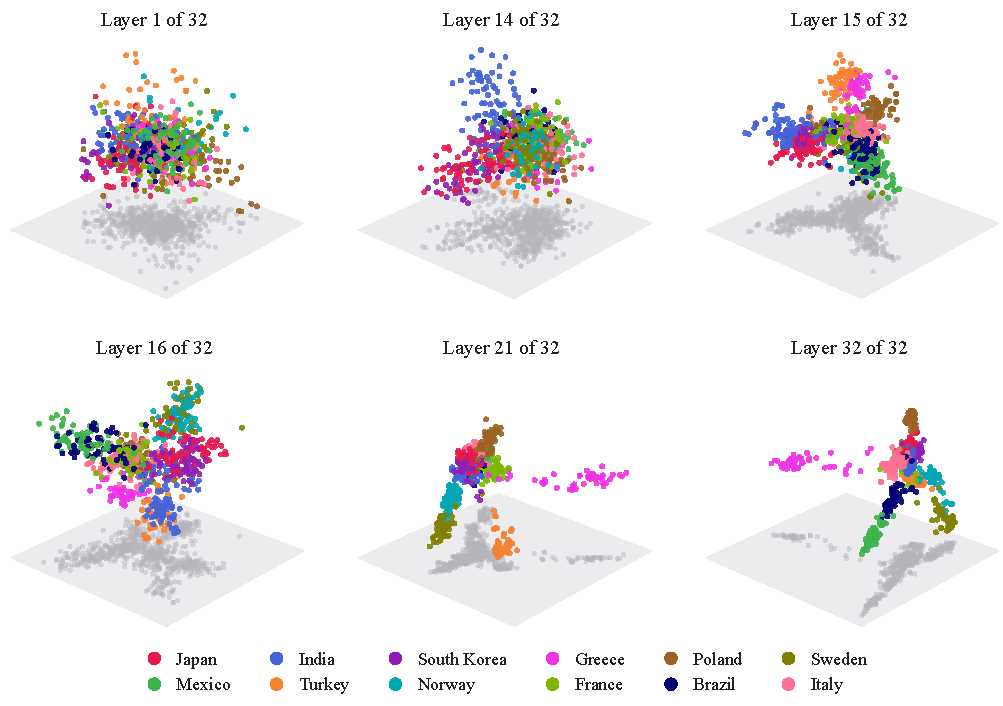
\includegraphics[width=\textwidth]{fig_hero.pdf}
\caption{\textbf{States of questions at six layers of Llama-3.1-8B.} Each point is one test question about a person, town or film whose answer is one of the twelve countries the model gave most often; colour is the country the model answered. Each panel shows the questions' states at one layer, projected onto the three directions that best separate the twelve countries among the training questions at that layer (found by linear discriminant analysis, LDA). At layer 1 all questions share one cloud, and at layer 14 a few countries, such as India, stand apart. At layer 15, where readability jumps (Section~\ref{sec:step}), most countries separate; by the last layer most form a strand of their own. Each panel is scaled separately; grey dots are shadows on the floor.}
\label{fig:hero}
\end{figure*}

\section{Methods}
\label{sec:setup}

\subsection{Questions}
To test whether questions with the same answer reach the same state, we need many different questions for each answer. We built such a set from Wikidata~\citep{vrandecic2014wikidata}. It has \NFacts{} facts and 62 possible answers of four kinds: 24 countries, 16 cities, 12 languages\footnote{We dropped Hindi as the language a person spoke after a manual check found its Wikidata labels unreliable. Hindi remains as the language of films.} and 10 sports. Each kind of answer is reached through one to three relations, or types of question. A country answers which country a person is a citizen of, which country a town is in, or which country a film is from. A city answers where a person was born or where a company is based. A language answers which language a person spoke or a film was made in. A sport answers which sport an athlete plays.

Models know popular facts far better than rare ones~\citep{mallen2022when}, so we sampled subjects evenly from three popularity bands (by number of Wikipedia language editions), giving a mix of facts the models know and do not know. Every subject has one value for its relation, a unique English label and no namesake of the same kind.

\subsection{Wordings and formats}
Each fact is asked as an open question in up to three wordings. One is a plain template: ``What country is An\'{i}bal Ponce a citizen of?'' Two are rewordings in assigned styles, such as a casual text or a quiz host's question: ``Hi, I'd appreciate knowing which country An\'{i}bal Ponce is a citizen of, if possible?'' A language model wrote the rewordings, knowing the subject but never the answer. We kept a rewording only if it named the subject exactly, asked a question, and mentioned no candidate answer or its demonym; \NRewrites{} passed.

The plain question is also asked as four-option multiple choice, in all four cyclic orders of the options. For a random 30\% of facts, it is also asked with a wrong suggestion from the user: ``In which country is Ireneo Portela? I'm fairly sure it's Mexico.'' In total, each model sees \NPromptsPerModel{} prompts in its own chat format.

\subsection{Models and recordings}
We study four instruction-tuned models: Llama-3.1-8B-Instruct~\citep{grattafiori2024the}, Qwen2.5-7B-Instruct~\citep{qwen2024qwen25}, Gemma-2-9B-it~\citep{gemma2024gemma} and Llama-3.2-1B-Instruct. All answer greedily.

A transformer builds its output in the residual stream, a vector at each token position that every layer reads and adds to. The answer is produced from the last position of the prompt, so we record the residual stream there before the first layer and after every layer (before the final normalisation). We call this vector the question's \emph{state} at that layer, written $h_q^{\ell}$ for question $q$ at layer $\ell$. It has one number per dimension of the residual stream, for example 4,096 in Llama-3.1-8B. Depth is the fraction of the model's layers that the state has passed through.

A free-form reply is graded by its first line. If that line names one candidate, matched against hand-curated names such as ``China'' or ``Mandarin'', the reply is right or wrong. A single answer outside the candidate list is wrong. Replies that hedge, refuse or name two answers are set aside as unclear.

\subsection{Training and test questions}
Several of our measurements first fit something to questions and then test it, for example the answer places defined next. To keep each test fair, fitting and testing use different questions. We split the subjects (the people, towns, films, companies and athletes) at random into two halves, once, and use the same split throughout. Questions about the first half are \emph{training questions}; questions about the second half are \emph{test questions}. Anything fitted uses only training questions, and every number we report is measured on test questions. We split by subject rather than by question because the several questions about one subject, in different wordings and formats, are close copies of each other.

\subsection{Answer places}
An answer's \emph{place} at a layer is the average state, at that layer, of the training questions to which the model gave that answer:
\begin{equation}
p_a^{\ell} = \frac{1}{|Q_a|} \sum_{q \in Q_a} h_q^{\ell},
\label{eq:place}
\end{equation}
where $Q_a$ is the set of training questions that the model answered with $a$. For example, the place of Argentina at layer 15 of Llama-3.1-8B is the average layer-15 state of the training questions that Llama answered with ``Argentina'', whether about a person, a town or a film, in any wording. We build a place only for an answer the model gave at least five times, for at least three different subjects.

Places are built from the answers the model gives, not from the true answers. A question that the model answers wrongly with ``Chile'' counts toward the place of Chile. This lets us ask, later, where wrong answers sit.

\subsection{Readability}
\label{sec:read}
Readability asks whether the answer the model gave can be identified from where its state lies. A state and a place are vectors of the same size, so we can measure the distance between them; no output probabilities are involved. For a test question $q$, we find the nearest place among answers of the same kind (for a country question, among the country places):
\begin{equation}
\hat{a}(q) = \operatorname*{arg\,min}_{a \in A_q} \big\lVert W(h_q^{\ell}) - W(p_a^{\ell}) \big\rVert,
\label{eq:read}
\end{equation}
where $A_q$ is the set of places of the question's kind and $W$ is a whitening, described below. Readability at a layer is the share of test questions for which $\hat{a}(q)$ is the answer the model gave, counting only questions whose given answer has a place. If states carried no information about the answer, readability would be about one over the number of places, for example 4\% for the 24 countries.

Plain distances would mislead, because a few dimensions of the residual stream take very large values and dominate any distance. The whitening $W$ prevents this. At each layer, it re-expresses a state in the 128 directions along which training states vary most, and rescales each direction to unit variance, so that each direction counts equally. To avoid amplifying noise, each variance is first shrunk by 10\% toward the average variance.

\subsection{Tightness}
Readability depends on the whitening. Tightness gives a second view that does not: it measures, in the model's own states, how closely test questions gather around their places compared with how far apart the places are. At each layer,
\begin{equation}
T^{\ell} = \frac{\frac{1}{N} \sum_{q} \lVert h_q^{\ell} - p_{a(q)}^{\ell} \rVert^2}{\frac{1}{|A|} \sum_{a \in A} \lVert p_a^{\ell} - \bar{p}^{\ell} \rVert^2}.
\label{eq:tight}
\end{equation}
The upper sum runs over the $N$ test questions whose given answer $a(q)$ has a place. $A$ is the set of places of one kind of answer, and $\bar{p}^{\ell}$ is their average. The numerator is the average squared distance of a question from its own place. The denominator is the average squared distance of a place from the centre of all places. A small $T$ means that questions sit close to their places relative to the distances between places. We compute both parts for each kind of answer and add them, weighting each kind by its number of test questions.

\subsection{Uncertainty and controls}
Questions about the same subject are not independent: a model tends to get all of them right or all of them wrong. We therefore measure uncertainty by resampling subjects. We draw test subjects at random, with replacement, 300 times, recompute the measure on the questions of the drawn subjects each time, and report the range that holds the middle 95\% of the results.

Two controls show how much readability could arise without information about the answer in the states. In the first, we shuffle the given answers between facts of the same kind before building places, and average over five shuffles. This keeps the number and sizes of the places but breaks the link between a state and its answer, so it measures readability by chance. In the second, we replace each state with a representation of the question's text alone: weighted counts of its two- to four-character sequences, reduced to 256 dimensions. This measures how much of the answer can be guessed from the wording, for example from the spelling of a name.

\section{Answers arrive in a step}
\label{sec:step}

Figure~\ref{fig:read}a shows how often the answer a model gives can be read from where its state is, layer by layer, for held-out questions. In every model the curve has the same shape: a low plateau, a jump within a few layers, and a high plateau. In Llama-3.1-8B readability rises from below 30\% to 71\% between layers 13 and 15 and reaches \PeakLlama{}; in Qwen2.5-7B the jump comes later, at layer \OnsetLayerQwen{} of 28, and reaches \PeakQwen{}. The depth of the jump differs between models (Table~\ref{tab:models}) but in each it is a sharp event, not a slow approach.

\begin{figure*}[t]
\centering
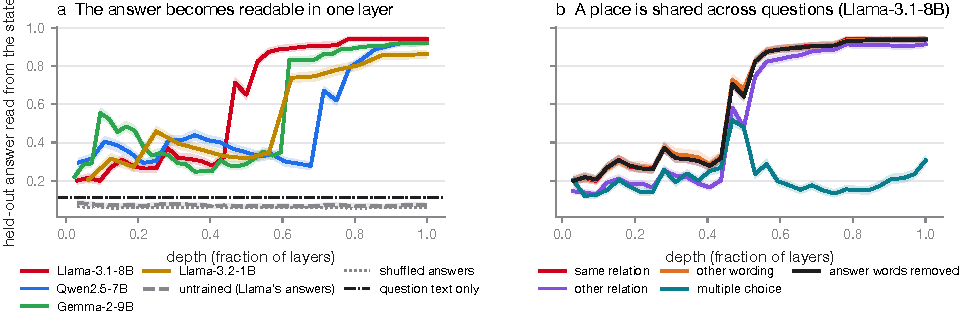
\includegraphics[width=\textwidth]{fig_decodability.pdf}
\caption{\textbf{Answers become readable at one depth, and what is read is a concept.} Held-out readability: the share of held-out questions whose nearest place (fitted on training subjects, same answer kind) is the answer the model gave; bands are 95\% intervals from resampling subjects. (a) All four models, with three controls: the same test on an untrained Llama-3.1-8B using the trained model's answers, labels shuffled between facts, and the question's text alone. (b) Llama-3.1-8B: places fitted on one relation and tested on the others (``other relation''); fitted on plain questions and tested on rewordings (``other wording''); with the answer words' output directions removed; and tested on the states of the multiple-choice version of the same questions.}
\label{fig:read}
\end{figure*}

The early plateau is not zero. Before the jump, 20--55\% of answers can be read, more than the shuffled control (\ShuffledLlama{}) and more than the question's text alone (\TextLlama{}--\TextQwen{}). We think this early signal reflects surface cues the model has already picked up from the subject's name, such as the language a name or title is in; we did not test this. Whatever its source, it does not grow with depth, and the jump goes far beyond it.

Three controls show that the structure is learned. An untrained Llama-3.1-8B, given the same prompts and grouped by the trained model's answers, never exceeds \UntrainedPeak{}. Shuffling answers between facts gives \ShuffledLlama{}--\ShuffledLlamaSmall{} at every layer. A classifier on the question's words alone reaches at most \TextQwen{}.

\paragraph{Tightness tells the same story.} Readability depends on a whitening of the state. The tightness ratio does not: it compares, in the model's own space, how far held-out questions sit from their place with how far places sit from each other. It falls 16- to 25-fold through the network (Figure~\ref{fig:tight}), and most of the fall happens at once. We fitted two shapes to the logarithm of each model's curve, a straight line (the same contraction at every layer, as seen in trained classifiers~\citep{he2022a}) and a single smooth step, and compared them by how well each predicts a left-out layer. The step wins in every model, by a factor of 5 to 24 in prediction error (Table~\ref{tab:models}).

\begin{figure}[t]
\centering
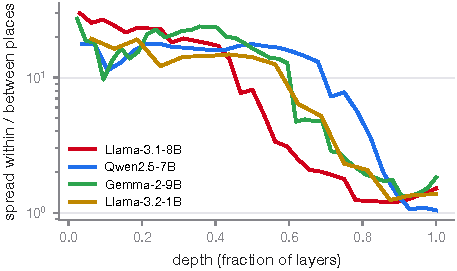
\includegraphics[width=\columnwidth]{fig_contraction.pdf}
\caption{\textbf{Tightness falls in a step.} Average squared distance of held-out questions from their place, divided by the spread of places, in each model's own space (log scale).}
\label{fig:tight}
\end{figure}

\begin{table}[t]
\centering
\footnotesize
\setlength{\tabcolsep}{2.6pt}
\begin{tabular}{@{}lcccc@{}}
\toprule
 & Llama 8B & Qwen 7B & Gemma 9B & Llama 1B \\
\midrule
Layers & \LayersLlama{} & \LayersQwen{} & \LayersGemma{} & \LayersLlamaSmall{} \\
Accuracy & \AccLlama{} & \AccQwen{} & \AccGemma{} & \AccLlamaSmall{} \\
Readable from (depth) & \OnsetLlama{} & \OnsetQwen{} & \OnsetGemma{} & \OnsetLlamaSmall{} \\
Peak readability & \PeakLlama{} & \PeakQwen{} & \PeakGemma{} & \PeakLlamaSmall{} \\
Error, step fit & \StepMseLlama{} & \StepMseQwen{} & \StepMseGemma{} & \StepMseLlamaSmall{} \\
Error, line fit & \LineMseLlama{} & \LineMseQwen{} & \LineMseGemma{} & \LineMseLlamaSmall{} \\
Other relation & \XRelLlama{} & \XRelQwen{} & \XRelGemma{} & \XRelLlamaSmall{} \\
Answer words removed & \NoWordsLlama{} & \NoWordsQwen{} & \NoWordsGemma{} & \NoWordsLlamaSmall{} \\
\bottomrule
\end{tabular}
\caption{\textbf{Per-model summary.} ``Readable from'': the layer, as a fraction of depth, at which readability first covers half the distance from chance to its peak, chosen on training subjects only. Step and line fits: mean squared error in predicting a left-out layer's log tightness. The last two rows are readability at 90\% of depth.}
\label{tab:models}
\end{table}

\section{A place is a concept, not a word}
\label{sec:concept}

If a place were only the model preparing to say a word, it would depend on how the question was asked and on the word's output direction. It depends on neither. A place fitted only on questions about people's citizenship finds the right country for questions about towns and films just as well: at 90\% of depth, \XRelLlama{} for Llama-3.1-8B, against \PeakLlama{} within the same relation (Figure~\ref{fig:read}b). Places fitted on plain questions work on casual or formal rewordings (\XWordLlama{}). And removing from the state every direction the output layer uses to write any of the 62 answer names, with the final normalisation's scaling taken into account, leaves readability unchanged (\NoWordsLlama{}); removing a random subspace of the same size does the same. The output layer does read these directions, so they are present, but the place does not depend on them.

The multiple-choice version of each question shows where the concept stops. When the options are listed and the model must answer with a letter, the content place is briefly readable from the multiple-choice state at the step (52\% in Llama-3.1-8B, against a shuffled level near 6\%), then fades to \ToMcqLlama{} as the state turns toward a letter. This matches the finding that models decide on the content of an option before binding it to its letter~\citep{wong2026when,wiegreffe2024answer}.

\section{Moving the state moves the answer}
\label{sec:steer}

Readability shows that the answer can be read from the place; it does not show that the model uses it. To test this we moved states. For a held-out question that the model answered wrongly, we added to its state, at one layer and at the last prompt position only, the difference between the right answer's place and the place of the answer it gave, and let the model answer again. As controls, we added a random direction of the same length, and we moved the state toward a third answer's place.

\begin{figure*}[t]
\centering
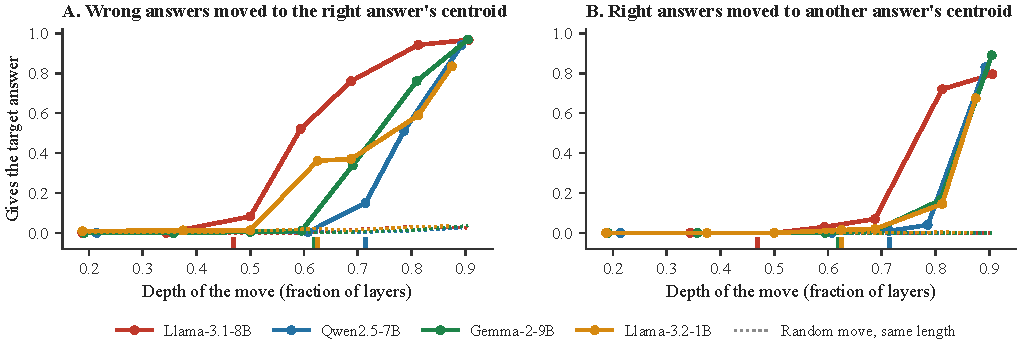
\includegraphics[width=\textwidth]{fig_steering.pdf}
\caption{\textbf{Moving a state into a place changes the answer, but only after the step.} (a) Wrong answers moved toward the right answer's place (solid) or by a random direction of the same length (dotted). (b) Right answers moved toward a different answer's place. The y-axis is the share of questions for which the model then gives the answer it was moved toward. Ticks under the axis mark the depth at which each model's answers become readable. Held-out questions; places from training subjects.}
\label{fig:steer}
\end{figure*}

The result follows the step (Figure~\ref{fig:steer}). Before a model's answers become readable, moves toward the right place do nothing: at 20\% of depth they correct \PushEarlyLlama{}--\PushEarlyLlamaSmall{} of wrong answers. After the step they work, and they work more the later they are made, reaching \PushGoldLlama{} (Llama-3.1-8B), \PushGoldQwen{} (Qwen2.5-7B), \PushGoldGemma{} (Gemma-2-9B) and \PushGoldLlamaSmall{} (Llama-3.2-1B) at about 90\% of depth. Random moves of the same length change \PushRandomLlama{}--\PushRandomGemma{} of these answers. The effect is not specific to the truth: moved toward a third answer's place, the model gives that answer \PushOtherQwen{}--\PushOtherGemma{} of the time, and right answers moved toward another place are given up for it \PushRightOtherLlamaSmall{}--\PushRightOtherGemma{} of the time. Each model follows the move only from the depth at which its own answers become readable, so the depth of the step measured by reading and the depth at which the model starts to act on the place agree.

Late moves are, in part, close to writing the answer directly, because late states are near the output. The informative parts of the experiment are the depth at which moves start to work, the failure of random moves, and the model's willingness to follow a move to any answer.

\section{Where wrong answers sit}
\label{sec:errors}

Because places are defined by what the model says, a wrong answer has a place too. At the depth where answers become readable, about half of the wrong answers that name a candidate sit nearest the place of the answer they gave (\AnatInGivenLlama{} for Llama-3.1-8B, \AnatInGivenQwen{} for Qwen2.5-7B), as confident mistakes, and \AnatInGoldLlama{} of all wrong answers sit nearest the right answer's place. This geometry carries information the output does not. For each wrong free-form answer we asked whether the model still picks the right option in the multiple-choice version (in more than half of the option orders it answered), and predicted this from the model's confidence in its reply, from the geometry of its state (distance to the right place, the right place's rank, and the margin to the nearest place), or from both, with five-fold cross-validation grouped by subject. Geometry predicts recognition better than confidence in every model (Figure~\ref{fig:errors}a): AUC \AucGeoLlama{} against \AucConfLlama{} for Llama-3.1-8B and \AucGeoGemma{} against \AucConfGemma{} for Gemma-2-9B, whose confidence carries no signal at all here. Adding geometry to confidence improves AUC in every model; the 95\% intervals for the gain, from resampling subjects, are \AucGainLoLlama{} to \AucGainHiLlama{} (Llama-3.1-8B), \AucGainLoQwen{} to \AucGainHiQwen{} (Qwen2.5-7B), \AucGainLoGemma{} to \AucGainHiGemma{} (Gemma-2-9B) and \AucGainLoLlamaSmall{} to \AucGainHiLlamaSmall{} (Llama-3.2-1B). The wrong answers studied number \ErrNLlama{}, \ErrNQwen{}, \ErrNGemma{} and \ErrNLlamaSmall{}.

\begin{figure*}[t]
\centering
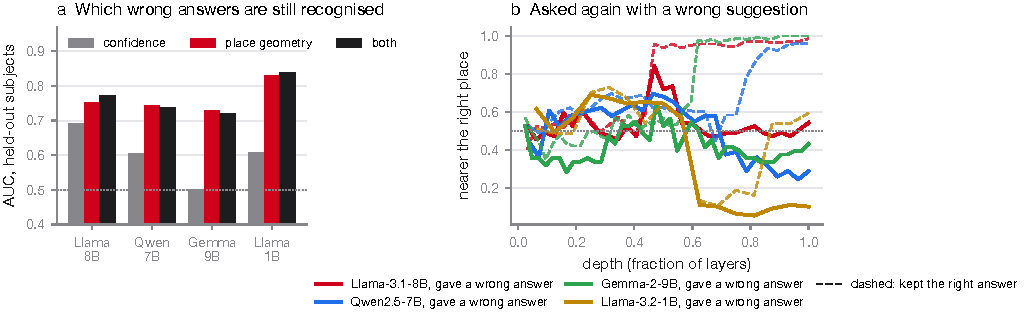
\includegraphics[width=\textwidth]{fig_errors.pdf}
\caption{\textbf{The geometry of a wrong answer says what the model still knows.} (a) Among wrong free-form answers on held-out subjects: how well the model's confidence in its reply, the geometry of its state at the step, or both, predict that it still picks the right option in multiple choice (AUC, five-fold cross-validation grouped by subject). (b) Questions answered correctly when asked plainly. With a user's wrong suggestion, those the model resisted (dashed) move to the right place and stay; those it was misled on (solid) first move toward the right place at the step, then away from it. Y-axis: share of states nearer the right answer's place than the suggested answer's place.}
\label{fig:errors}
\end{figure*}

The hint condition shows the same geometry in a case where we know what happened. For questions a model answers correctly when asked plainly, adding ``I'm fairly sure it's \dots'' with a wrong country sometimes changes the answer. Where the model resists, its state goes to the right place at the step and stays there (\HintResistEndLlama{} of states nearer the right place at the last layer of Llama-3.1-8B). Where the model is misled, the state first goes toward the right place too, with up to \HintPeakLlama{} of these states nearer it than the suggested place at about half depth, and then leaves it (\HintEndLlama{} at the last layer; \HintEndQwen{} in Qwen2.5-7B). Moving such a misled state back to the right place restores the right answer \PushMisledLlama{} of the time in Llama-3.1-8B. The model reached the answer it knew, and later layers replaced it.

\paragraph{Places hold beliefs.} Two models sometimes give different answers to the same question. If places reflected the question rather than the model's answer, both models' states would sit near the same place. They do not: in all \CrossModelPairs{} ordered pairs of models, on questions where the two disagree, each model's state is nearer its own answer's place than the other model's answer's place in \CrossModelMin{}--\CrossModelMax{} of cases.

\section{Related work}
\label{sec:related}

\paragraph{Reading intermediate layers.}
The logit lens~\citep{nostalgebraist2020interpreting} decodes an intermediate state through the model's output layer, and the tuned lens~\citep{belrose2023eliciting} learns a decoder for each layer. Both show predictions sharpening with depth. Future Lens~\citep{pal2023future} and Patchscopes~\citep{ghandeharioun2024patchscopes} read richer content from a single hidden state. All of these read the state through the output vocabulary. Our places are fitted from the states themselves, and reading them does not need the answer words' output directions.

\paragraph{How depth is used.}
Several studies find that layers play different roles. Early layers gather and detokenise, middle layers build abstract features, and late layers refine a prediction~\citep{lad2024the,csordas2025do,gupta2025how,cheng2024emergence,skean2025layer}. Correct and incorrect predictions follow similar confidence curves across layers~\citep{kim2025on}. In factual recall, information about the relation and then the subject moves to the last position, where attention heads extract the attribute~\citep{geva2023dissecting}. Feed-forward layers act as key--value memories~\citep{geva2020transformer}, and middle-layer feed-forward modules at the subject's last token are causally decisive~\citep{meng2022locating}. Our onset depth marks, for a whole population of questions, the depth at which each model's answer becomes available at the last position.

\paragraph{Representation geometry.}
Middle layers represent the same content in a shared space across languages and modalities~\citep{wendler2024do,wu2024the}. Concepts have structured geometry. Categories form simplices~\citep{park2024the}, some features are circular~\citep{engels2024not}, space and time are linearly decodable~\citep{gurnee2023language}, counts lie on curved manifolds that attention reshapes~\citep{gurnee2026when}, and truth has a linear direction~\citep{marks2023the}. In trained classifiers, representations of different classes separate by a roughly constant factor per layer~\citep{he2022a}. Language models move partway toward neural collapse, in which states gather at their class means, at their top layer, and further with scale~\citep{wu2024linguistic}. The residual stream contains stable regions, within which small changes leave the next-token prediction unchanged~\citep{janiak2024characterizing}. Yet, almost surely, no two prompts map to the same last-position state~\citep{nikolaou2025language}. Places fit both findings: questions can gather in the directions that carry the answer while staying distinct in others.

\paragraph{What models know but do not say.}
Internal states often encode more than the output shows~\citep{orgad2024llms,gekhman2025insideout,ruscio2026on}. On knowledge benchmarks such as MMLU and ARC, however, this gap is near zero~\citep{park2025bridging}, and internal states mostly reflect what the model recalls rather than what is true~\citep{cheang2026do}. False few-shot demonstrations can override a correct internal answer at a critical layer~\citep{halawi2023overthinking}, and users' suggestions shift answers~\citep{sharma2023towards}. In multiple choice, attention in a few middle layers selects the answer letter, and a sparse set of heads then raises its probability~\citep{wiegreffe2024answer}. The winning option is chosen by its content before it is bound to its letter~\citep{wong2026when}, and models carry a prior over letters~\citep{zheng2023large}.

\paragraph{Steering.}
Adding a direction to the residual stream changes a model's behaviour~\citep{panickssery2023steering,li2023inferencetime}. Our moves are of this kind. Each one, however, takes a single question's state from one measured place to another at one layer, and is compared with random moves of the same length.

\section{Limitations}
\label{sec:limits}

The questions are factual and short, and their answers come from a closed set of 62 countries, cities, languages and sports; three of the four kinds are names, and for the one kind that is not (sports) the jump is much smaller and late readability lower, so whether places behave the same way for common nouns in general is open. Places for open-ended answers, multi-step reasoning or long contexts may look different. We studied four instruction-tuned models between 1 and 9 billion parameters, one prompt format each, and greedy answers. Readability uses a whitening of the state; the tightness ratio does not, and it falls fastest at the same depth, but both measure where states sit, not the computation that moves them there. The step fit compares two simple shapes; it shows that a sudden change describes the data much better than a constant contraction, not that the change happens within a single layer. Moves at late layers partly write the answer directly, so the strongest causal evidence is the depth at which moves start to work and the failure of random moves. Wikidata answers are a reference, not ground truth; we removed one unreliable relation--answer pair after a manual check, and a small number of wrong labels surely remain. The rewordings were written by a language model and filtered automatically.

\section{Conclusion}
\label{sec:conclusion}

For the first half to two thirds of each network, the state from which the answer is produced carries only a weak trace of the answer, and moving it almost never changes the answer to the right one. At one layer the answer arrives. From that layer on, every question with the same answer sits near one centroid, whatever was asked, and moving a state to another centroid changes the reply. Wrong answers are placed the same way, so a near miss can be seen at the onset as a right answer that came second. We have not tested larger models, or open-ended answers, which have no fixed set of centroids; these are the obvious next cases.


\paragraph{Code and data.} Code, the dataset and all derived results: \url{https://github.com/gut-puncture/The-Shape-of-Wisdom}.

\paragraph{Acknowledgements.} This work was inspired by Goodfire's Neural Geometry series~\citep{goodfire2026the}. The questions come from Wikidata~\citep{vrandecic2014wikidata}. Language models (Claude, GPT and Fable) helped with literature review, code review and drafting; all experiments, numbers and claims were checked against the recorded data.


\small
\bibliographystyle{plainnat}
\bibliography{references}

\end{document}
